\chapter{Results and Discussion}

\section{Design Results}
All six joints size correctly, satisfy every applicable failure check, generate every component as a solid model and produce a drawing sheet. Each design completes in approximately ten seconds. Table~\ref{tab:joints} summarises the results.

\begin{table}[htbp]
\centering\footnotesize
\caption{Design results for the six joints at the duties adopted}\label{tab:joints}
\begin{tabularx}{\textwidth}{>{\raggedright\arraybackslash}X>{\raggedright\arraybackslash}Xrr>{\raggedleft\arraybackslash}p{2.4cm}>{\raggedright\arraybackslash}p{2cm}}
\toprule
Joint & Duty adopted & Parts & Checks & Busiest check, \% of allowable & Outcome \\
\midrule
Knuckle joint & Load P = 50,000 N & 5 & 9 & 79 & all satisfied \\
Socket and spigot cotter joint & Load P = 35,000 N & 3 & 10 & 76 & all satisfied \\
Sleeve and cotter joint & Load P = 50,000 N & 5 & 8 & 77 & all satisfied \\
Gib and cotter joint & Load P = 50,000 N & 4 & 8 & 79 & all satisfied \\
Hex bolt, nut and washer & Load P = 20,000 N & 3 & 2 & 71 & all satisfied \\
Protected type rigid flange coupling & Torque T = 500,000 N mm (500 N m) & 12 & 7 & 79 & all satisfied \\
\bottomrule
\end{tabularx}
\end{table}


The busiest check across the six joints lies between 71 and 79 percent of the allowable stress. That range is the intended consequence of the design factor described in Section~5.4 and confirms that margin is retained in every case.

\section{Worked Example}
The requirement \emph{knuckle joint for 50 kN} is interpreted as the knuckle joint carrying an axial load of 50,000 N with the default allowable stresses. Applying the design factor, the joint is sized for 62,500 N. Table~\ref{tab:raw} gives the governing calculations.

\begin{table}[htbp]
\centering\footnotesize
\caption{Governing calculations for a knuckle joint carrying 50 kN, before rounding}\label{tab:raw}
\begin{tabularx}{\textwidth}{Xrl}
\toprule
Expression & Computed, mm & Effect \\
\midrule
Rod in direct tension & 32.57 & rod diameter adopted as 35 mm \\
Pin in double shear & 25.75 & not governing \\
Pin in bending & 44.85 & governs; pin diameter adopted as 45 mm \\
\bottomrule
\end{tabularx}
\end{table}


The rod requirement of 32.57 mm is rounded up to the adopted 35 mm. The pin requirement arising from bending (44.85 mm, adopted as 45 mm) is about 1.74 times that arising from shear (25.75 mm). A pin sized from shear alone would satisfy its own check and bend in service, which is why the larger of the two requirements is adopted, as the source material does. Table~\ref{tab:dims} gives the complete set of dimensions with the rule and the source behind each.

\begin{table}[htbp]
\centering\scriptsize
\caption{Dimensions computed for the knuckle joint, with the rule behind each}\label{tab:dims}
\begin{tabularx}{\textwidth}{>{\raggedright\arraybackslash}p{1.3cm}>{\raggedright\arraybackslash}p{3.6cm}r>{\raggedright\arraybackslash}X}
\toprule
Symbol & Meaning & Value, mm & Rule and source \\
\midrule
\texttt{D} & rod diameter & 35 & rod in tension: D = sqrt(4P / (pi sigma\_t)), rounded up to a preferred size \\
\texttt{d} & pin diameter & 45 & governed by pin bending \\
\texttt{d2} & eye outer diameter & 90 & d2 = 2.0 x d, the pin diameter (outer diameter of eye and fork, d0 = 2d), rounded up to a standard size [Bhandari, Design of Machine Elements, sec 4.12, eq 4.26j] \\
\texttt{d3} & pin head and collar diameter & 70 & d3 = 1.5 x d, the pin diameter (pin head and collar diameter, 1.5d), rounded up to a standard size [Bhandari, Design of Machine Elements, sec 4.12, eq 4.26o] \\
\texttt{D1} & enlarged end, 1.1D & 40 & D1 = 1.1 x D, the rod diameter (enlarged rod diameter near the eye and fork, D1 = 1.1D), rounded up to a standard size [Bhandari, Design of Machine Elements, sec 4.12, eq 4.26b] \\
\texttt{t} & eye thickness & 45 & t = 1.25 x D, the rod diameter (thickness of eye of rod B, b = 1.25D), rounded up to a standard size [Bhandari, Design of Machine Elements, sec 4.12, eq 4.26n] \\
\texttt{t1} & fork plate thickness & 30 & t1 = 0.75 x D, the rod diameter (thickness of each fork eye, a = 0.75D), rounded up to a standard size [Bhandari, Design of Machine Elements, sec 4.12, eq 4.26m] \\
\texttt{t2} & pin head thickness & 18 & t2 = 0.5 x D, the rod diameter (thickness of pin head), rounded up to a whole mm [NPTEL IIT KGP M4L2 fig 4.2.3.1] \\
\texttt{collar\_t} & collar thickness & 23 &  \\
\texttt{taper\_d} & taper pin diameter (big end) & 9 &  \\
\bottomrule
\end{tabularx}
\end{table}


With all dimensions determined, the nine failure modes are evaluated at the actual load of 50,000 N. The results are given in Table~\ref{tab:checks}. Every check is satisfied, and the busiest, bending of the pin, reaches 79 percent of its allowable stress.

\begin{table}[htbp]
\centering\footnotesize
\caption{Failure checks for the knuckle joint, evaluated at the actual load of 50 kN}\label{tab:checks}
\begin{tabularx}{\textwidth}{>{\raggedright\arraybackslash}p{2.4cm}>{\raggedright\arraybackslash}Xrrr>{\raggedright\arraybackslash}p{1.2cm}}
\toprule
Failure mode & Expression & Stress, MPa & Allowable, MPa & Utilisation, \% & Result \\
\midrule
rod tension & \texttt{4P / (pi D\^{}2)} & 51.969 & 75 & 69 & safe \\
pin double shear & \texttt{P / (2 pi/4 d\^{}2)} & 15.719 & 60 & 26 & safe \\
pin bending & \texttt{32M / (pi d\^{}3), M = P/2 (t1/3 + t/4)} & 59.3829 & 75 & 79 & safe \\
eye tension & \texttt{P / ((d2 - d) t)} & 24.6914 & 75 & 33 & safe \\
eye shear & \texttt{P / ((d2 - d) t)} & 24.6914 & 60 & 41 & safe \\
eye crushing & \texttt{P / (d t)} & 24.6914 & 150 & 16 & safe \\
fork tension & \texttt{P / ((d2 - d) 2 t1)} & 18.5185 & 75 & 25 & safe \\
fork shear & \texttt{P / ((d2 - d) 2 t1)} & 18.5185 & 60 & 31 & safe \\
fork crushing & \texttt{P / (d 2 t1)} & 18.5185 & 150 & 12 & safe \\
\bottomrule
\end{tabularx}
\end{table}


\begin{landscape}
\begin{figure}
\centering
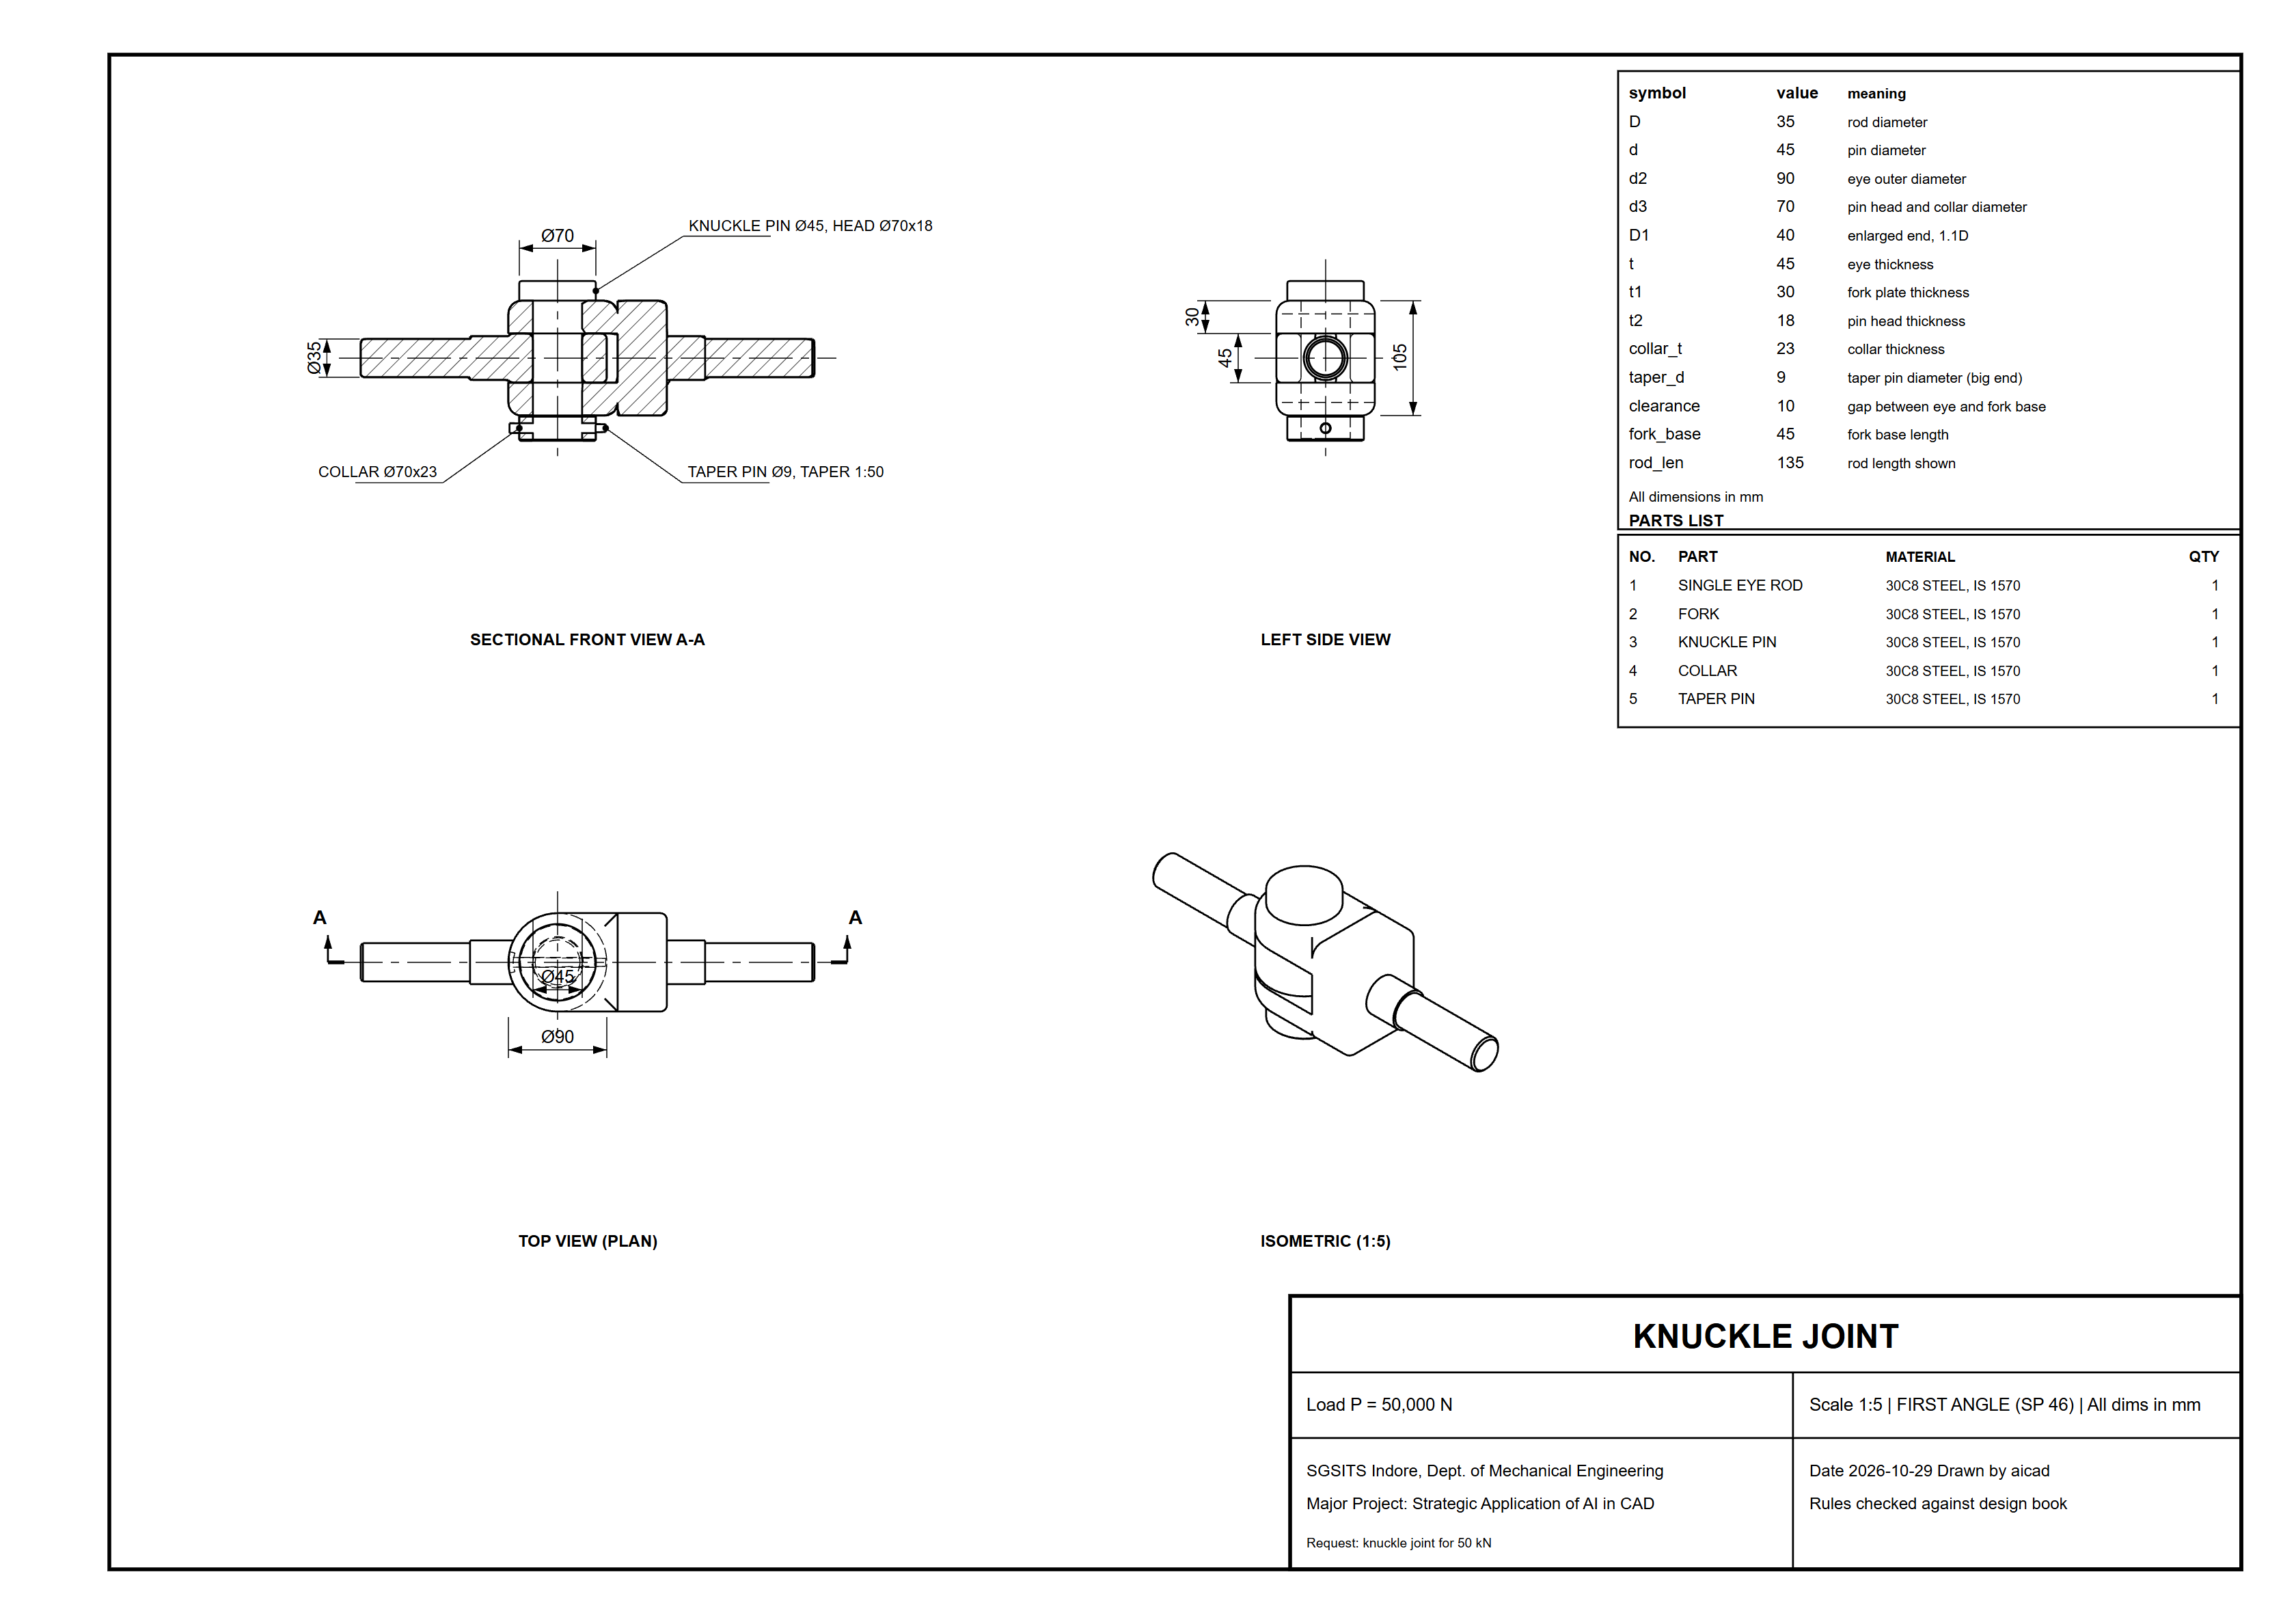
\includegraphics[width=\linewidth,height=0.94\textheight,keepaspectratio]{fig/drawing.png}
\caption{First angle A3 drawing sheet for the knuckle joint of Section 7.2: sectional front view A-A, side view, plan, isometric, parts list}
\label{fig:drawing}
\end{figure}
\end{landscape}

\begin{figure}
\centering
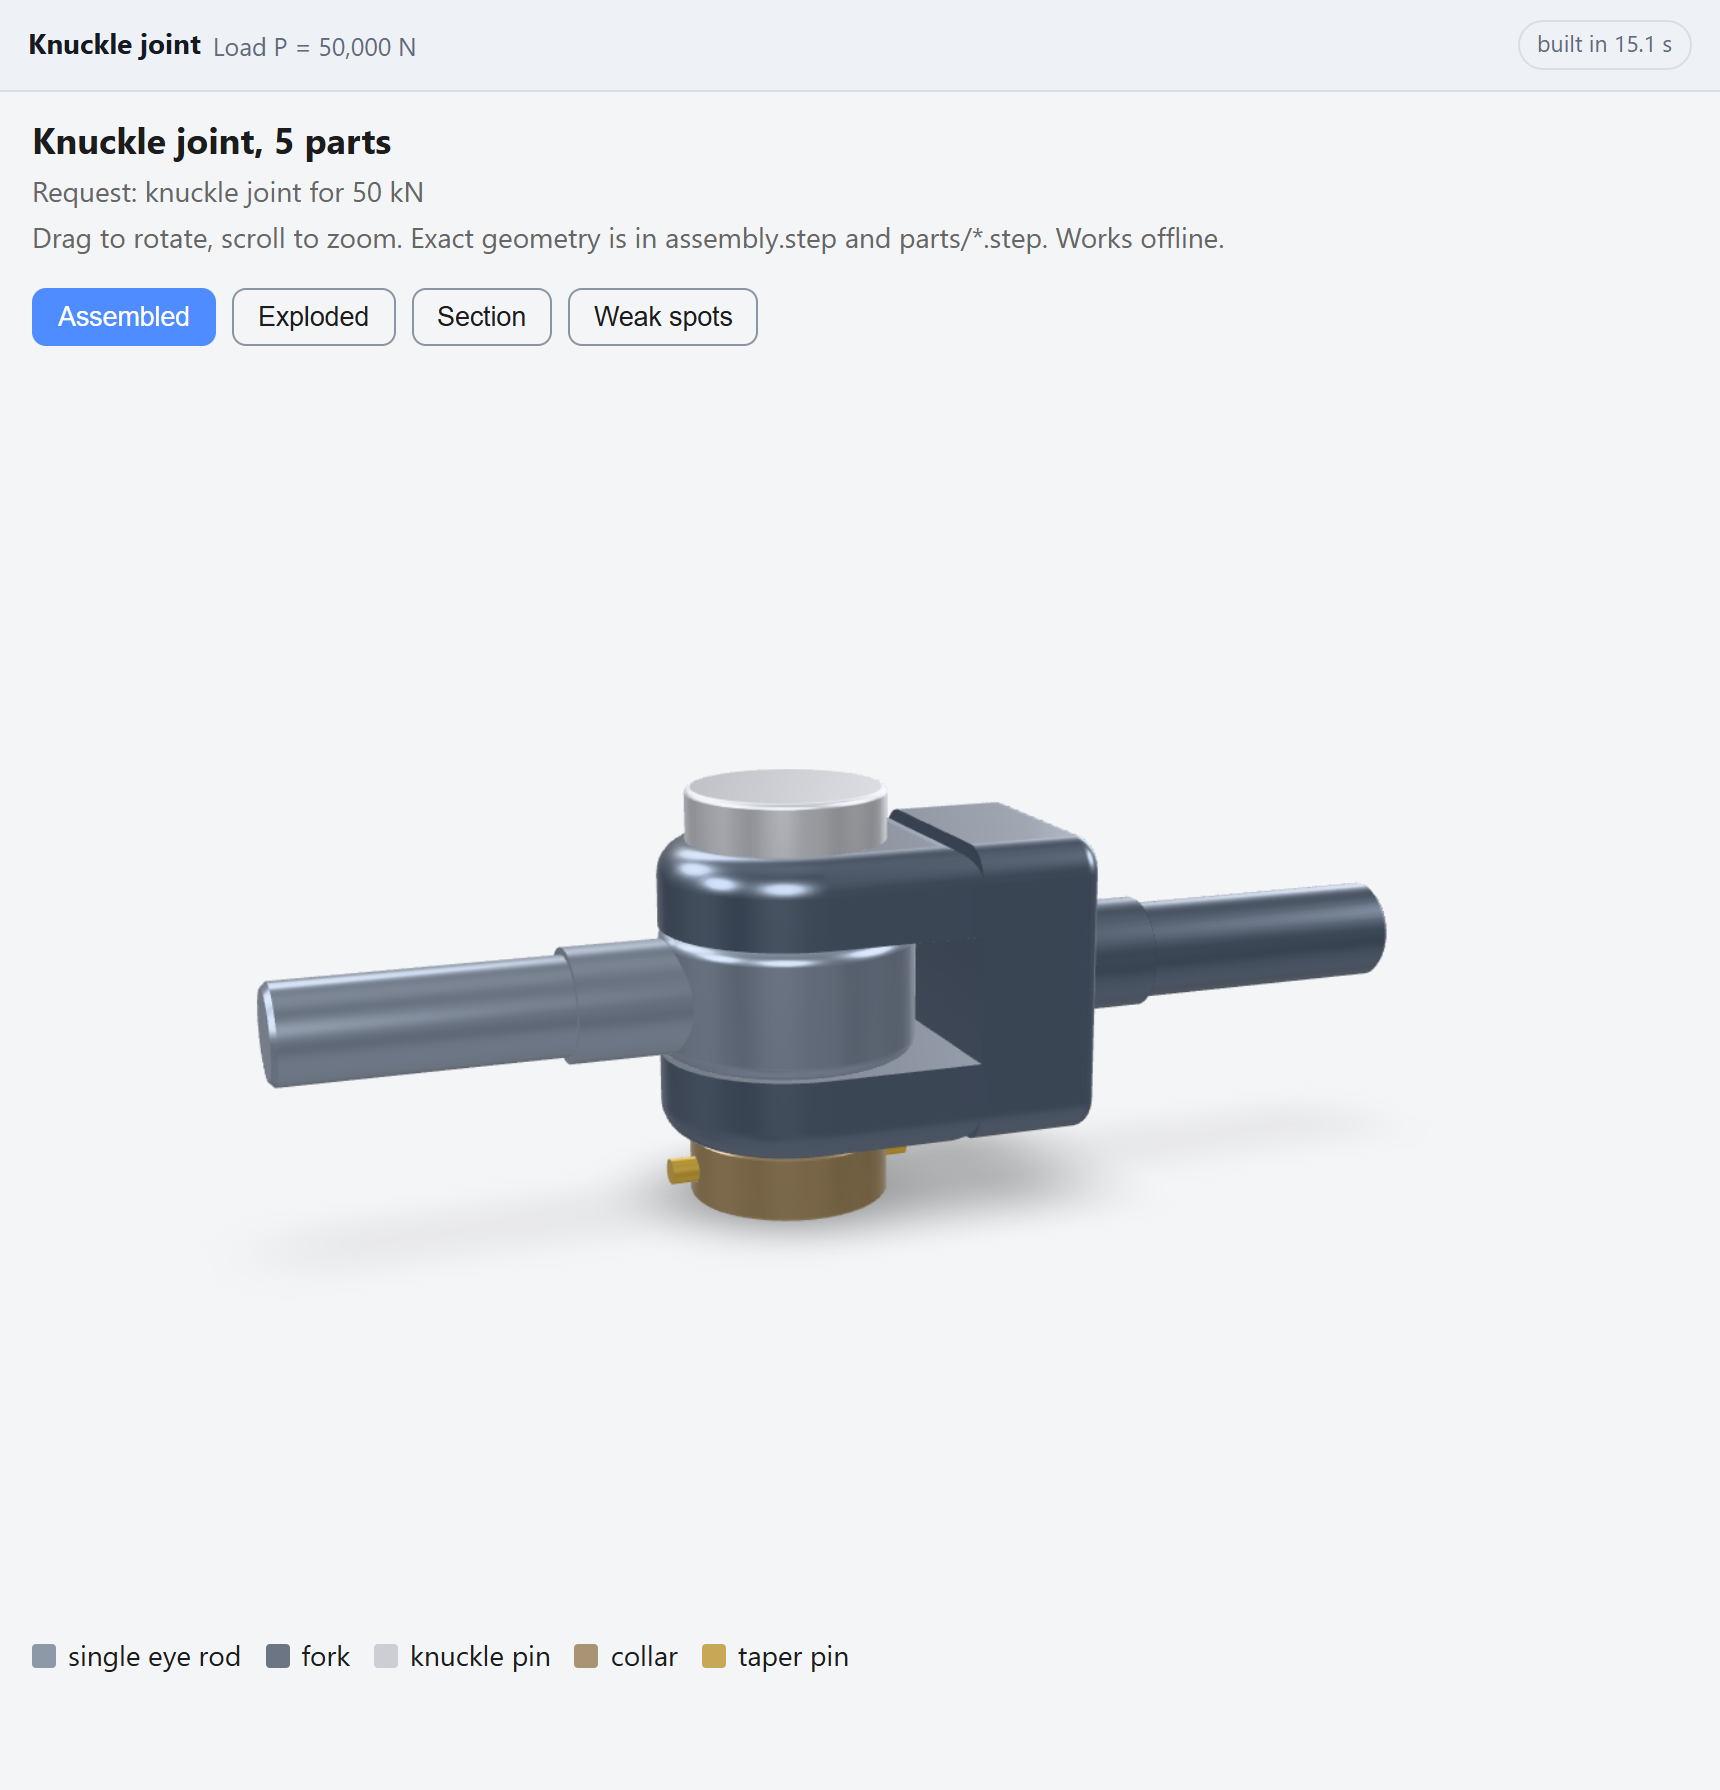
\includegraphics[width=0.62\textwidth]{fig/model.png}
\caption{Assembled model of the same joint, also available exploded and coloured by utilisation}
\label{fig:model}
\end{figure}

\section{Verification Against Published Literature}
Every proportion and every failure check was compared against the sources reviewed in Chapter~2. The outcome for each joint is given in Table~\ref{tab:verify}.

\begin{table}[htbp]
\centering
\caption{Verification of each joint against published design literature}
\label{tab:verify}
\small
\begin{tabularx}{\textwidth}{@{}lXX@{}}
\toprule
Joint & Source consulted & Outcome \\
\midrule
Knuckle joint & Bhandari Ex 4.5 and Problem 4.1; NPTEL Module 4 Lesson 2 & Sizes and stresses of Ex 4.5 reproduced exactly; all checks verified \\
Socket and spigot cotter & Bhandari Ex 4.2; NPTEL Module 4 Lesson 2; Leutwiler Art.\ 98 & Nine of ten sizes reproduced; checks verified against two sources \\
Gib and cotter & Unwin, p.\ 179 & Breadth division, thickness and taper verified \\
Protected flange coupling & NPTEL Module 4 Lesson 1; Leutwiler Art.\ 275 & All checks verified twice; proportions not verifiable \\
Sleeve and cotter & Four sources searched, none covers it & Checks verified by correspondence; proportions unverified \\
Hex bolted joint & NPTEL Module 4 Lesson 4 & Tightening relation verified; size table unverified \\
\bottomrule
\end{tabularx}
\end{table}

Two entries require explanation. For the flange coupling, the failure checks are verified against two independent sources, but the empirical proportions are marked unverified. This is not an omission. As recorded in Section~2.2, Leutwiler states that no standard set of proportions was ever agreed and that published tables reflect the practice of individual manufacturers. The proportions are therefore a convention, and the system reports them as such on every run. For the sleeve and cotter joint, none of four sources treats the joint by name; its checks are verified by direct correspondence with the socket and spigot cotter joint, but its proportions remain unsupported and are reported as such.

The strongest test is the reproduction of complete worked examples. Given the inputs of Bhandari's Example 4.5, the software adopts all seven sizes the book adopts and computes the same six eye and fork stresses, 31.25 and 25 N/mm\textsuperscript{2}. Table~\ref{tab:bhandari} sets the two side by side.

\begin{table}[htbp]
\centering\footnotesize
\caption{Bhandari Example 4.5 (50 kN, 30C8, factor of safety 5) against the software run with the same inputs}\label{tab:bhandari}
\begin{tabularx}{\textwidth}{llrrl}
\toprule
Quantity & Meaning & Book & Software & Agrees \\
\midrule
\texttt{D} & rod diameter & 30 & 30 & yes \\
\texttt{D1} & enlarged end, 1.1D & 35 & 35 & yes \\
\texttt{t} & eye thickness & 40 & 40 & yes \\
\texttt{t1} & fork plate thickness & 25 & 25 & yes \\
\texttt{d} & pin diameter & 40 & 40 & yes \\
\texttt{d2} & eye outer diameter & 80 & 80 & yes \\
\texttt{d3} & pin head and collar diameter & 60 & 60 & yes \\
eye tension & stress, MPa & 31.25 & 31.25 & yes \\
fork tension & stress, MPa & 25 & 25 & yes \\
\bottomrule
\end{tabularx}
\end{table}


Problem 4.1 is reproduced to the printed 14.47 mm for the rod and 13.47 mm for the pin. For the cotter joint of Example 4.2, nine of the ten adopted sizes agree, including the spigot and socket diameters solved from their tension equations (37.91 and 52.04 mm before rounding). The one difference, the width of the cotter, follows from the book designing the cotter alone with a factor of safety of 4 while the software applies the factor of the rods to every part. Each of these cases is an automated test and a one click case in the web application.

The two texts also disagree on one proportion of the knuckle joint. The NPTEL lesson takes the pin head as 1.5 times the rod diameter, which gives 60 mm on its own 55 mm pin, a head only 5 mm larger than the pin. Bhandari takes it as 1.5 times the pin diameter. The software follows Bhandari.

\section{Discrepancies Found in the Sources}
The verification exercise identified three errors in the published sources. They are recorded here because the behaviour of the system deliberately differs from the printed material in consequence.

\subsection{A Worked Example That Fails Its Own Check}
The NPTEL knuckle joint problem raises the pin diameter from 40 mm to 55 mm to satisfy bending, but then evaluates the eye using the original 40 mm pin. Evaluated with the pin actually adopted, its own expression for shear of the eye gives 80 MPa against an allowable of 65 MPa, an exceedance of 23 percent. The present system instead enlarges the outer diameter of the eye and reports that it has done so.

\subsection{An Omitted Failure Mode}
The NPTEL cotter joint procedure verifies crushing of the socket but not crushing between the cotter and the spigot. Evaluated at the final answer of that source, the omitted check gives 167 MPa against an allowable of 110 MPa. Leutwiler, in Article 98, lists this mode among ten, with an expression of identical form. The present system retains the check and sizes the cotter thicker in consequence. That an independent text, published eighteen years earlier, lists a check which the lesson omits establishes this as an omission rather than a matter of preference.

\subsection{A Constant Printed Incorrectly}
The initial tightening load for a bolted joint is printed as $284d$ kN. The worked example on the same page obtains 56.8 kN for an M20 bolt, which is consistent only with a constant of $2840d$ N. The printed relation is therefore in error by a factor of one hundred, and the source refutes itself. The system uses $2840d$ N and reports the tightening load on every bolted design.

\section{Finite Element Comparison}
The finite element facility was first validated against a case with a known answer. Table~\ref{tab:fe} gives the comparison, measured on the September geometry.

\begin{table}[htbp]
\centering
\caption{Comparison of the finite element result with the calculated stress}
\label{tab:fe}
\small
\begin{tabularx}{\textwidth}{@{}>{\raggedright\arraybackslash}Xrrr@{}}
\toprule
Case & Formula, MPa & FEA, MPa & Diff., \% \\
\midrule
Bar of 20 mm diameter, 10 kN in tension & 31.83 & 32.22 & $+1.2$ \\
Knuckle joint eye rod, 50 kN & 52.0 & 57.9 & $+11.3$ \\
\bottomrule
\end{tabularx}
\end{table}

The bar validates the method. The eye rod reads higher because the calculation treats the rod as a plain bar in tension and takes no account of the stress raised at the pin bore, whereas the finite element model does. Both values remain below the allowable stress of 75 MPa.

The convergence rule described in Section~5.7 proved necessary in practice. For one component the computed peak varied from 157 to 191 MPa across a sixteen fold increase in the number of nodes without settling, which indicates a singularity at the constrained face rather than a physical stress. The system reports such a result as not converged and directs the user to the calculated value.

\section{Discussion}
The division of responsibility of Section~5.2 gave a natural language interface without making any part of the design unverifiable, and printing the arithmetic of every check is what exposed the three discrepancies of Section~7.4: each surfaced because a computed number disagreed with a printed one.

\section{Objectives Revisited}
\begin{enumerate}
\item \textbf{Interpreting a plain English requirement.} Met. The language model extracts the joint type and load, as shown in Section~5.2, and any value it returns that cannot be traced back to the original sentence is discarded, which guards against a fabricated input.
\item \textbf{Sizing and verifying against every failure mode, with iteration.} Met. All six joints satisfy every applicable check at the stated load, as given in Table~\ref{tab:joints}, and the iterative enlargement of Section~5.5 is what makes the gib and cotter strap, and the knuckle eye of the NPTEL problem, pass where the source proportions alone would not.
\item \textbf{Exact solid models in a neutral format that opens in commercial CAD software.} Substantially met. Every exported assembly was inspected directly and confirmed to carry the AUTOMOTIVE\_DESIGN (AP214) schema with each component as a separate named solid rather than a single fused body, which is the structure Siemens NX requires to recognise an assembly on import. Opening the file inside NX itself, available only in the departmental laboratory, is the one point not yet confirmed by direct observation and is recorded as such.
\item \textbf{A first angle drawing sheet conforming to Indian practice.} Met for projection and sheet layout, as shown in Figure~\ref{fig:drawing}. Dimensioning to SP 46 tolerance and surface finish conventions is not implemented and is listed in Section~8.2.
\item \textbf{Verification against published literature, with disagreements recorded.} Met for four of six joints and partially met for the remaining two, as tabulated in Table~\ref{tab:verify}. The three discrepancies of Section~7.4 are the direct product of this objective rather than a side finding.
\item \textbf{Browser use without installation.} Met. The system is deployed and reachable without a local install, though the hosted copy runs the rule based interpreter rather than the language model, a distinction recorded in Section~5.2.
\end{enumerate}

